% Options for packages loaded elsewhere
\PassOptionsToPackage{unicode}{hyperref}
\PassOptionsToPackage{hyphens}{url}
\PassOptionsToPackage{dvipsnames,svgnames,x11names}{xcolor}
\documentclass[
  10pt,
  fontset=fandol]{ctexart}
\usepackage{xcolor}
\usepackage[margin=16mm]{geometry}
\usepackage{amsmath,amssymb}
\setcounter{secnumdepth}{-\maxdimen} % remove section numbering
\usepackage{iftex}
\ifPDFTeX
  \usepackage[T1]{fontenc}
  \usepackage[utf8]{inputenc}
  \usepackage{textcomp} % provide euro and other symbols
\else % if luatex or xetex
  \usepackage{unicode-math} % this also loads fontspec
  \defaultfontfeatures{Scale=MatchLowercase}
  \defaultfontfeatures[\rmfamily]{Ligatures=TeX,Scale=1}
\fi
\usepackage{lmodern}
\ifPDFTeX\else
  % xetex/luatex font selection
\fi
% Use upquote if available, for straight quotes in verbatim environments
\IfFileExists{upquote.sty}{\usepackage{upquote}}{}
\IfFileExists{microtype.sty}{% use microtype if available
  \usepackage[]{microtype}
  \UseMicrotypeSet[protrusion]{basicmath} % disable protrusion for tt fonts
}{}
\makeatletter
\@ifundefined{KOMAClassName}{% if non-KOMA class
  \IfFileExists{parskip.sty}{%
    \usepackage{parskip}
  }{% else
    \setlength{\parindent}{0pt}
    \setlength{\parskip}{6pt plus 2pt minus 1pt}}
}{% if KOMA class
  \KOMAoptions{parskip=half}}
\makeatother
\usepackage{graphicx}
\makeatletter
\newsavebox\pandoc@box
\newcommand*\pandocbounded[1]{% scales image to fit in text height/width
  \sbox\pandoc@box{#1}%
  \Gscale@div\@tempa{\textheight}{\dimexpr\ht\pandoc@box+\dp\pandoc@box\relax}%
  \Gscale@div\@tempb{\linewidth}{\wd\pandoc@box}%
  \ifdim\@tempb\p@<\@tempa\p@\let\@tempa\@tempb\fi% select the smaller of both
  \ifdim\@tempa\p@<\p@\scalebox{\@tempa}{\usebox\pandoc@box}%
  \else\usebox{\pandoc@box}%
  \fi%
}
% Set default figure placement to htbp
\def\fps@figure{htbp}
\makeatother
\setlength{\emergencystretch}{3em} % prevent overfull lines
\providecommand{\tightlist}{%
  \setlength{\itemsep}{0pt}\setlength{\parskip}{0pt}}
\usepackage{amsmath,amssymb,mathtools,needspace}
\xeCJKDeclareCharClass{CJK}{"2032,"0400->"04FF,"2160->"216B,"2460->"2473,"25A0,"25C7,"25CB,"25CF}
\IfFontExistsTF{Arial Unicode MS}{\xeCJKsetup{AutoFallBack=true}\setCJKfallbackfamilyfont{\CJKrmdefault}{Arial Unicode MS}}{}
\setcounter{secnumdepth}{0}
\setlength{\emergencystretch}{2em}
\allowdisplaybreaks
\usepackage{bookmark}
\IfFileExists{xurl.sty}{\usepackage{xurl}}{} % add URL line breaks if available
\urlstyle{same}
\hypersetup{
  pdftitle={Walsh 阵的演化机制},
  colorlinks=true,
  linkcolor={Maroon},
  filecolor={Maroon},
  citecolor={Blue},
  urlcolor={Blue},
  pdfcreator={LaTeX via pandoc}}

\title{Walsh 阵的演化机制}
\author{}
\date{}

\begin{document}
\maketitle

\subsubsection{10.3.3　Walsh 阵的演化机制}\label{walsh-ux9635ux7684ux6f14ux5316ux673aux5236}

Walsh 阵的演化方式从属于二分演化模式。事实上，这里从初态 \(W_1=[+]\) 出发，将 \(W_{N/2}\) 加工成 \(W_N\) 的二分手续如下。

（1）分裂手续。

\href{../../source-images/pdf-268.jpeg}{原页}

对 \(W_{N/2}\) 的每一行 \(W_{N/2}(i)\) 分别施行偶复制与奇复制，生成两个 \(N\) 维向量 \([W_{N/2}(i)\mathrel{\vdots}\ddot W_{N/2}(i)]\) 与 \([W_{N/2}(i)\mathrel{\vdots}\dot W_{N/2}(i)]\)。

（2）合成手续。

将 \(W_{N/2}\) 的每一行按上述分裂手续扩展为相邻的两个 \(N\) 维向量，从而将 \(W_{N/2}\) 扩展成为一个 \(N\) 阶方阵

\[
W_N=\begin{pmatrix}
\vdots&\vdots\\
W_{N/2}(i)\mathrel{\vdots}&\ddot W_{N/2}(i)\\
W_{N/2}(i)\mathrel{\vdots}&\dot W_{N/2}(i)\\
\vdots&\vdots
\end{pmatrix},
\]

如此反复地做下去。这种二分演化机制如图 10.3 所示。如 10.1.2 小节所看到的，Walsh 函数的表达式很复杂，直接利用表达式生成 Walsh 函数很困难。然而依据上述镜像行复制的演化方式，一蹴而就地派生出一个又一个 Walsh 方阵，从而得到一族又一族 Walsh 函数。Walsh 函数的数目是逐族倍增的，这是一种快速生成算法。

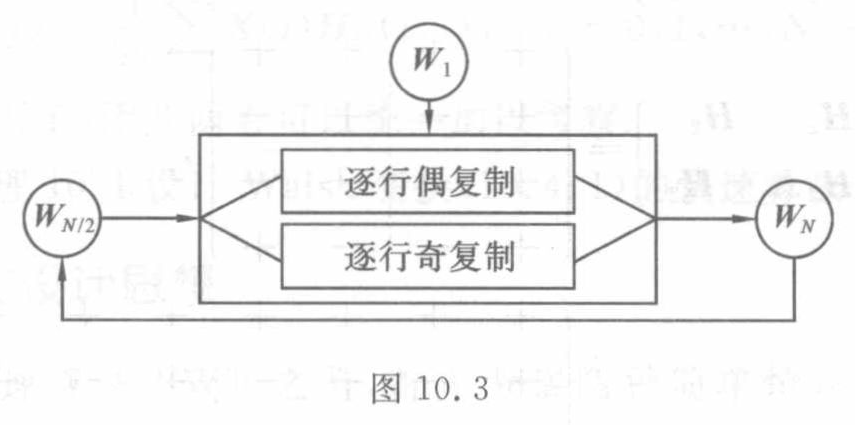
\includegraphics[width=0.85\linewidth,height=\textheight,keepaspectratio,alt={图 10.3（原图裁切）：Walsh 阵的二分演化机制}]{../assets/ch10/fig-10-3.png}

图 10.3

\begin{quote}
图中文字与图意（转录）：初态 \(W_1\) 从上方进入；\(W_{N/2}\) 分成``逐行偶复制''和``逐行奇复制''两路，合成为 \(W_N\)；\(W_N\) 经下方反馈线返回 \(W_{N/2}\)。
\end{quote}

\end{document}
